\documentclass[preprint, 3p,
authoryear]{elsarticle} %review=doublespace preprint=single 5p=2 column
%%% Begin My package additions %%%%%%%%%%%%%%%%%%%

\usepackage[hyphens]{url}

  \journal{An awesome journal} % Sets Journal name

\usepackage{graphicx}
%%%%%%%%%%%%%%%% end my additions to header

\usepackage[T1]{fontenc}
\usepackage{lmodern}
\usepackage{amssymb,amsmath}
% TODO: Currently lineno needs to be loaded after amsmath because of conflict
% https://github.com/latex-lineno/lineno/issues/5
\usepackage{lineno} % add
\usepackage{ifxetex,ifluatex}
\usepackage{fixltx2e} % provides \textsubscript
% use upquote if available, for straight quotes in verbatim environments
\IfFileExists{upquote.sty}{\usepackage{upquote}}{}
\ifnum 0\ifxetex 1\fi\ifluatex 1\fi=0 % if pdftex
  \usepackage[utf8]{inputenc}
\else % if luatex or xelatex
  \usepackage{fontspec}
  \ifxetex
    \usepackage{xltxtra,xunicode}
  \fi
  \defaultfontfeatures{Mapping=tex-text,Scale=MatchLowercase}
  \newcommand{\euro}{€}
\fi
% use microtype if available
\IfFileExists{microtype.sty}{\usepackage{microtype}}{}
\usepackage[]{natbib}
\bibliographystyle{plainnat}

\ifxetex
  \usepackage[setpagesize=false, % page size defined by xetex
              unicode=false, % unicode breaks when used with xetex
              xetex]{hyperref}
\else
  \usepackage[unicode=true]{hyperref}
\fi
\hypersetup{breaklinks=true,
            bookmarks=true,
            pdfauthor={},
            pdftitle={Short Paper},
            colorlinks=false,
            urlcolor=blue,
            linkcolor=magenta,
            pdfborder={0 0 0}}

\setcounter{secnumdepth}{5}
% Pandoc toggle for numbering sections (defaults to be off)

% Pandoc syntax highlighting
\usepackage{color}
\usepackage{fancyvrb}
\newcommand{\VerbBar}{|}
\newcommand{\VERB}{\Verb[commandchars=\\\{\}]}
\DefineVerbatimEnvironment{Highlighting}{Verbatim}{commandchars=\\\{\}}
% Add ',fontsize=\small' for more characters per line
\usepackage{framed}
\definecolor{shadecolor}{RGB}{248,248,248}
\newenvironment{Shaded}{\begin{snugshade}}{\end{snugshade}}
\newcommand{\AlertTok}[1]{\textcolor[rgb]{0.94,0.16,0.16}{#1}}
\newcommand{\AnnotationTok}[1]{\textcolor[rgb]{0.56,0.35,0.01}{\textbf{\textit{#1}}}}
\newcommand{\AttributeTok}[1]{\textcolor[rgb]{0.13,0.29,0.53}{#1}}
\newcommand{\BaseNTok}[1]{\textcolor[rgb]{0.00,0.00,0.81}{#1}}
\newcommand{\BuiltInTok}[1]{#1}
\newcommand{\CharTok}[1]{\textcolor[rgb]{0.31,0.60,0.02}{#1}}
\newcommand{\CommentTok}[1]{\textcolor[rgb]{0.56,0.35,0.01}{\textit{#1}}}
\newcommand{\CommentVarTok}[1]{\textcolor[rgb]{0.56,0.35,0.01}{\textbf{\textit{#1}}}}
\newcommand{\ConstantTok}[1]{\textcolor[rgb]{0.56,0.35,0.01}{#1}}
\newcommand{\ControlFlowTok}[1]{\textcolor[rgb]{0.13,0.29,0.53}{\textbf{#1}}}
\newcommand{\DataTypeTok}[1]{\textcolor[rgb]{0.13,0.29,0.53}{#1}}
\newcommand{\DecValTok}[1]{\textcolor[rgb]{0.00,0.00,0.81}{#1}}
\newcommand{\DocumentationTok}[1]{\textcolor[rgb]{0.56,0.35,0.01}{\textbf{\textit{#1}}}}
\newcommand{\ErrorTok}[1]{\textcolor[rgb]{0.64,0.00,0.00}{\textbf{#1}}}
\newcommand{\ExtensionTok}[1]{#1}
\newcommand{\FloatTok}[1]{\textcolor[rgb]{0.00,0.00,0.81}{#1}}
\newcommand{\FunctionTok}[1]{\textcolor[rgb]{0.13,0.29,0.53}{\textbf{#1}}}
\newcommand{\ImportTok}[1]{#1}
\newcommand{\InformationTok}[1]{\textcolor[rgb]{0.56,0.35,0.01}{\textbf{\textit{#1}}}}
\newcommand{\KeywordTok}[1]{\textcolor[rgb]{0.13,0.29,0.53}{\textbf{#1}}}
\newcommand{\NormalTok}[1]{#1}
\newcommand{\OperatorTok}[1]{\textcolor[rgb]{0.81,0.36,0.00}{\textbf{#1}}}
\newcommand{\OtherTok}[1]{\textcolor[rgb]{0.56,0.35,0.01}{#1}}
\newcommand{\PreprocessorTok}[1]{\textcolor[rgb]{0.56,0.35,0.01}{\textit{#1}}}
\newcommand{\RegionMarkerTok}[1]{#1}
\newcommand{\SpecialCharTok}[1]{\textcolor[rgb]{0.81,0.36,0.00}{\textbf{#1}}}
\newcommand{\SpecialStringTok}[1]{\textcolor[rgb]{0.31,0.60,0.02}{#1}}
\newcommand{\StringTok}[1]{\textcolor[rgb]{0.31,0.60,0.02}{#1}}
\newcommand{\VariableTok}[1]{\textcolor[rgb]{0.00,0.00,0.00}{#1}}
\newcommand{\VerbatimStringTok}[1]{\textcolor[rgb]{0.31,0.60,0.02}{#1}}
\newcommand{\WarningTok}[1]{\textcolor[rgb]{0.56,0.35,0.01}{\textbf{\textit{#1}}}}

% tightlist command for lists without linebreak
\providecommand{\tightlist}{%
  \setlength{\itemsep}{0pt}\setlength{\parskip}{0pt}}

% From pandoc table feature
\usepackage{longtable,booktabs,array}
\usepackage{calc} % for calculating minipage widths
% Correct order of tables after \paragraph or \subparagraph
\usepackage{etoolbox}
\makeatletter
\patchcmd\longtable{\par}{\if@noskipsec\mbox{}\fi\par}{}{}
\makeatother
% Allow footnotes in longtable head/foot
\IfFileExists{footnotehyper.sty}{\usepackage{footnotehyper}}{\usepackage{footnote}}
\makesavenoteenv{longtable}






\begin{document}


\begin{frontmatter}

  \title{Short Paper}
    \author[Some Institute of Technology]{Irina Vélez%
  \corref{cor1}%
  \fnref{1}}
   \ead{alice@example.com} 
    \author[Another University]{Otto Palkama%
  %
  \fnref{1}}
   \ead{bob@example.com} 
      \affiliation[Some Institute of Technology]{
    organization={Big Wig University},addressline={1 main
street},city={Gotham},postcode={123456},state={State},country={United
States},}
    \affiliation[Another University]{
    organization={Department},addressline={A street
29},city={Manchester,},postcode={2054 NX},country={The Netherlands},}
    \cortext[cor1]{Corresponding author}
    \fntext[1]{This is the first author footnote.}
    \fntext[2]{Another author footnote.}
  
  \begin{abstract}
  This is the abstract.

  It consists of two paragraphs.
  \end{abstract}
    \begin{keyword}
    keyword1 \sep 
    keyword2
  \end{keyword}
  
 \end{frontmatter}

\hypertarget{introduction}{%
\section{1. Introduction}\label{introduction}}

The idea is to explore how the use of Large Language Models (LLMs) as
General Purpose Technology (GPT) could reshape industries, considering
the generalization capabilities of LLMs and the rapid adoption of these
tools by the public and firms.

A. Background on the potential economic impact of Large Language Models
(LLMs) as General Purpose Technology (GPT) B. Objective of the paper:
Exploring how the use of LLMs as GPT could reshape industries and
contribute to economic growth

Generalization of tools seems to be an important characteristic to
leverage the potential of growth and development, because if a same tool
could be broad use for different purposes, so the tool becomes in a very
valuable tool.

Until now the abilities reached by the Large Languages Models LLMs have
arisen to a certain level of computational power that might require
scaling up past this threshold (10\^{}23 training FLOPs), meaning that
they are able to perform multiple tasks related to Text Understanding
and Generation,Problem Solving and Mathematics, Image and Data
Classification, Text Analysis and Comprehension, and so on, but as
\citep{weiemergent} suggested for future works, it could be possible new
abilities could emerge scaling up the models and understanding how
emergence occurs would provide new insights into how to train
more-capable language models.

On the other hand, the use of LLMs as a base technology of other tools,
such as software-AI powered, open a new window and enveloped the
potential of productivity improvements of the work-human force or human
capital as it was mention by \citep{gptaregpts} telling that LLMs such
as GPTs exhibit traits of general-purpose technologies, could have
considerable economic, social, and policy implications.

So, the potential arising of emergent abilities and the wide use of LLMs
as enablers of new tools (AI based-software) alongside the spread use of
tools such as ChatGPT by a large amount of humans (here: million of
users of chatGPT), it could signify a future unseen before by the human
beings, because the expansion and pushing of new boarders and limits
would be accelerated.

\hypertarget{generalization-capabilities-of-llms-as-gpt}{%
\section{Generalization Capabilities of LLMs as
GPT}\label{generalization-capabilities-of-llms-as-gpt}}

A. Examining the adoption rate of previous GPTs B. Key factors
contributing to the widespread adoption of a technology as a GPT C.
Reviewing the literature on the potential of AI as a GPT

Artificial intelligence a term coined by emeritus Stanford Professor
John McCarthy in 1955, was defined by him as ``the science and
engineering of making intelligent machines''.\footnote{Available at:
  https://hai.stanford.edu/sites/default/files/2020-09/AI-Definitions-HAI.pdf}
These systems are designed to simulate human cognitive abilities, such
as learning, reasoning, problem-solving, perception, and language
understanding. Within the realm of AI, Large Language Models (LLMs) are
a specific type of AI model that utilizes deep learning techniques,
particularly neural networks, to process and generate human-like
language. LLMs are trained on vast amounts of text data and can perform
tasks like language translation, text summarization, and question
answering.

In the past, computer programs were developed by painstakingly encoding
human knowledge, following a precise set of instructions that mapped
specific inputs to desired outputs. This approach required programmers
to meticulously define every step of the process. However, machine
learning systems operate differently. They utilize general algorithms,
such as neural networks, which enable them to independently determine
the appropriate mapping between inputs and outputs. This is achieved
through exposure to extensive datasets containing numerous examples. By
analyzing and learning from these examples, machine learning systems can
identify patterns and make accurate predictions or classifications
without explicit programming instructions.

General Purpose Technology is a transformative technology with a strong
improvement process at the begining and eventually becoming widely
adopted for its multiples uses, while producing many spillover effects
\citep{paradox}. As such, it have a pervasive impact on society as a
whole, mainly due to its capability to redefine the ways in which
businesses operate, improve productive and contribute to long-term
economic growth. Some well-know examples are steam power, electricity,
semiconductors, and internet.

Is it the AI a General Purpose Technology?

\hypertarget{what-is-the-potential-economic-impact-of-ai}{%
\section{What is the potential Economic Impact of
AI?}\label{what-is-the-potential-economic-impact-of-ai}}

What we are trying to do is following:

So, during times of structural changes as now, is difficult to see the
results of this new technologies, because the contributions in growth
that the successfull firms could make as offset by the decreases profits
of the outgoing firms. And this is why I think that the statistics is
not yet reflecting the potential benefits of the use of AI.

This can be ilustrated in Figure N, where the increases in investment,
are still not reflecting their fruits in increasings in the total factor
of productivity TFP.

\begin{itemize}
\tightlist
\item
  Graph of Investments during the last 10 years and TFP in the US.
  -Index of readiness to use AI by country
\end{itemize}

The intangible assets associated with the last wave of computerization
were about ten times as large as the direct investments in computer
hardware itself. paradox We think it is plausible that AI-associated
intangibles could be of a comparable or greater magnitude.

\begin{center}\rule{0.5\linewidth}{0.5pt}\end{center}

Considering the potential of the AI as a new GPT, specifically the LLMs,
assessing its potential contribution to the economic growth is worthy
during fast-pace changing times as now. The uncertainty's winds are
everywhere and setting expectations might be useful. Given the
uncertainty condition and the poor accuracy of predictions, assessing
its potential impact seems to be lead only by a retrospective approach,
what it means that the performance of previous General Purpose
Technology like steam power, electricity or internet, might give a more
realistic answer to this question.

However, this topic have already addressed by \citep{paradox} and
\citep{Nicholas}, in a context where are optimists and pessimists about
technology and growth. It arises a genuine dichotomy between higher
profit expectations of forward looking entrepreneurs, and the poor
growth performance reflected in the the backward looking statistics.

One example mentioned by \citep{paradox} is the call center industry,
which had approximately 2.2 million agents in 2015 in the United States.
It was plausible at that time to anticipate that voice recognition
systems like IBM's Watson could potentially reduce the number of workers
by 60\%. However, in hindsight, it is evident that the expectations have
not been fully met, as shown in Figure \ref{fig1}, which illustrates the
statistics.

\begin{figure}

{\centering 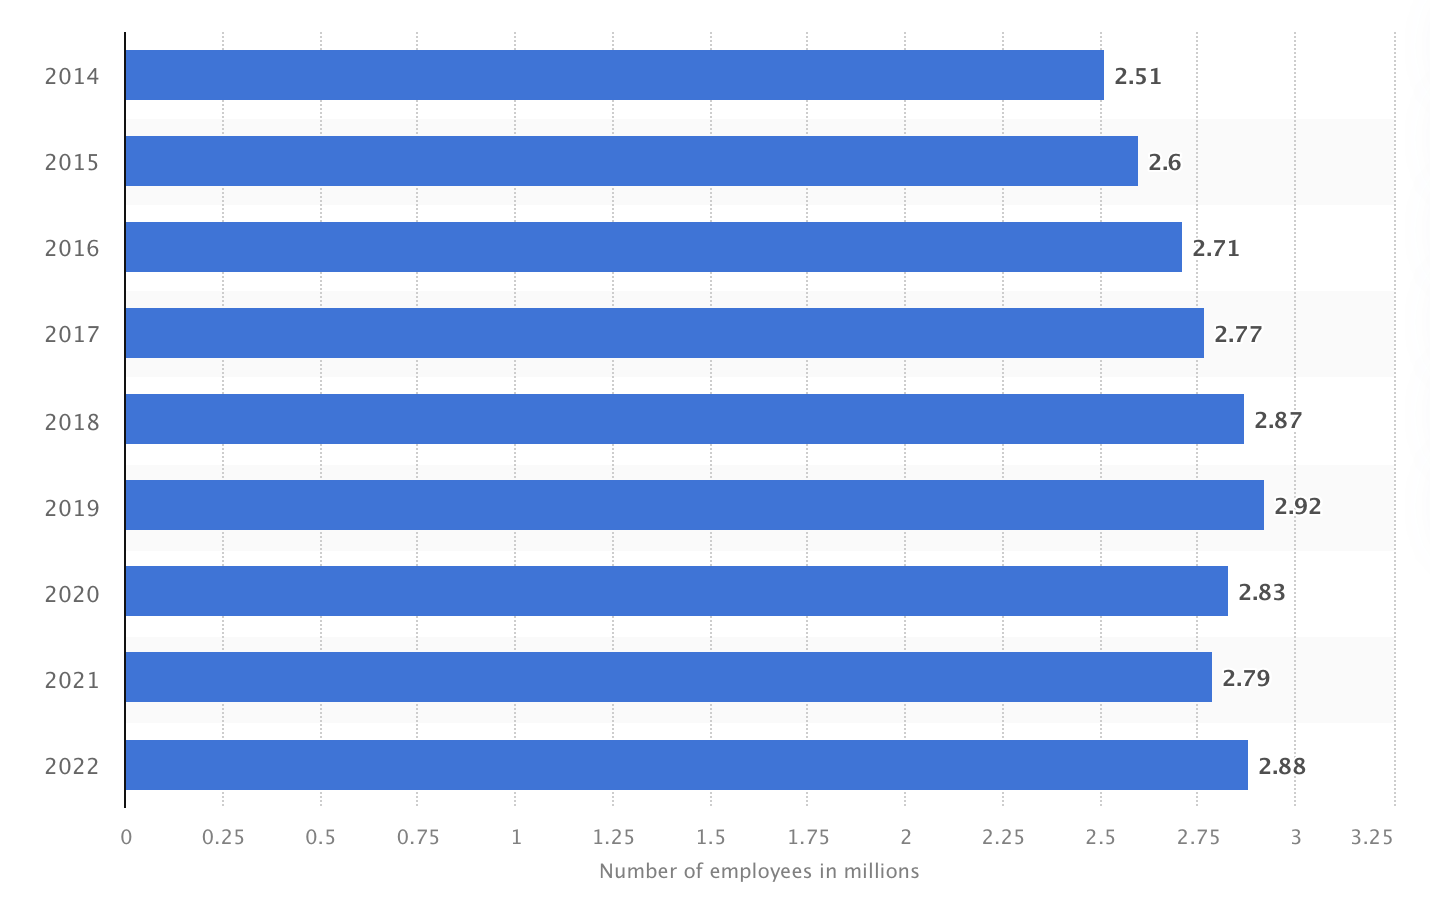
\includegraphics[width=0.7\linewidth]{../Views/contact_center_employees_US} 

}

\caption{\label{fig1}Number on contact center employees in the United States from 2014 to 2022.}\label{fig:fig1}
\end{figure}

As \citep{paradox} explain, this apparent incongruence relies on the
time lag between the technology creation and the full realization of its
benefits on the economy and society. It takes time to build the stock of
the new technology, develop the necessary human capital skillset,
undergo the re-engineering process of business process transformations,
and develop complementary innovations for its full realization in the
real economy.

To support this lag explanation, the Schumpeterian Growth Model might
give another good perspective, taking as a starting point that real
contributions to growth are value creation and cost optimization, so the
AI should be at the service of those growth contributors.

\hypertarget{gauging-the-potential-economic-impact-of-ai-in-terms-of-value-creation-and-cost-optimization}{%
\subsection{Gauging the potential economic impact of AI in terms of
value creation and cost
optimization}\label{gauging-the-potential-economic-impact-of-ai-in-terms-of-value-creation-and-cost-optimization}}

-Here, we are going to associate production function with creation of
value and cost optimization with the constraint which it is subject the
problem of maximization profits.

From one of the elemental problems of the economics, but fundamental for
growth, which corresponds to the firm's profit maximization, it can
derivate the two main goals of the private business sector: the
adjustment of their production function subjected to a constraint, that
in the most cases is a limited budget. So, for one side of the coin the
value creation contribute to get more from the production function, and
for the other side cost optimization aim to offset budget restrictions.
In this way, in terms of growth, the AI may be oriented toward one or
both of this goals.

From an economic perspective, one of the fundamental problems for growth
in firms is profit maximization. This goal leads to two main objectives
in the private business sector: adjusting the production function while
facing constraints, often in the form of a limited budget. Thus, on one
side of the coin, value creation contributes to maximizing output from
the production function, while on the other side, cost optimization aims
to mitigate budget restrictions. In terms of growth, AI can be directed
towards achieving one or both of these goals.

From one of the elemental problems in economics, but basic for economic
growth, it is the profit maximization firm's goal, which can be
represented as follows: \[
Profit = Total Income - Total Costs: \Pi = PX - C(X)
\] \[
Maximization Problem: \max_{x} \Pi(X) = PX - (wL + rK)
\] Where PX represents the revenue generated by the production function
X, and C(X) represents the corresponding costs associated to the costs
of labor and capital. This maximization problem leads to two main goals
in the private business sector: adjusting their production function X
while facing constraints C(X), often in the form of a limited budget.
Thus, on one side of the coin, value creation contributes to maximizing
output from the production function side, while on the other side, cost
optimization aims to mitigate not only budget restrictions, but also
limited resources.

To exemplify AI value creation, consider the use of deep neural network
systems in diagnosing skin cancer \citep{cancer}, detecting fraud and
assessing risks in the financial sector, and automating inventory
forecasting, as seen in Amazon's AI-Powered Inventory Management. On the
other hand, from a cost optimization perspective, AI is employed in
predictive maintenance and quality control to anticipate equipment
failures\footnote{Available at:
  https://www.ge.com/research/project/predictive-maintenance}.

\hypertarget{the-shumpenters-concept-of-creative-destruction}{%
\subsection{The Shumpenter's concept of creative
destruction}\label{the-shumpenters-concept-of-creative-destruction}}

Creative destruction refers to the process of creating and developing
new technology that continuously disrupt and replace the existing
obsolete technology in order to drive economic progress and
growth.\footnote{Definition created with the help of
  \href{https://github.com/mukulpatnaik/researchgpt.git}{ResearchGPT}}.

So, consider 2 types of firms, whose are creators of new technology and
great investors in Research and Development R\&D, such as big-tech
players like Apple, Amazon, Meta or Google, let's called Technology
``Creators'', and on the other side, firms which adopt and implement the
new technology in order to maximize their profits through the more value
added created by their production functions and cost optimization, or
both, let's called Technology ``Adopters''.

Knowledge or innovation is considered a \textbf{public good}, one you
have invented something , it becomes almost free of charge to
disseminate it through the world.{[}\^{}4{]} So, the first initial cost
of producing the technology have to be covered through monopolistic
profits (Creators), because this have been the mechanism that the market
system have found to coverage the huge initial costs.

A country with an amount R of resources can destine some of them
(Creators) toward doing R\&D, while others (Adopters) to produce a
certain level of activity or outcome X.

Creators: The proportion n is doing R\&D: \(nR\) Adopters: The remaining
is going to output X: \((1-n)R\)

If those firms are thought as a compound of human capital, the creators
are individuals with the skillset needed to create new technology, while
the adopters are individuals with enough skillset in produce X in the
traditional business model. Now, as

\begin{itemize}
\tightlist
\item
  Now introducing the concept of creative destruction, is explained by
  the fact that the process of destruction takes time from the
  perspective of the firms which need to adopt the new technology to
  receive its benefits. This means, that although the new technology (AI
  or LLM) have already free to use to the public, the maturity level of
  the other consumer firms should be evolve to be able to incorporate
  the new technology in their business process in an effective way such
  as it produces benefits to the firm. This destruction is explained in
  the Schumpeterian Growth Model for the monopolist by the expected days
  that the firm will remain in business if they don't adapt {[}tao{]}.
  This tao or time, is decreased by the increasing of productivity
  (gamma) and the deployment of new technologies (N). At the end this
  means transitional escenarios:
\item
  If the adopter firm are not able to incorporate the new technologies
  or take advantange of it, their profit will be diminishing until a
  possible exit of the market, when its proftis will be cero, and thsus,
  this firm won't contribute to the growth of the economy
\item
  If the adopter firm are able to incorporate the new technology or take
  advantange of it, their profit will increase, which in tur assurance
  their permanence in the market. However, this profit is not
  inmediatly. It takes time, due to the adaptation of their business
  process, the upskillset of their human capital, the time required for
  the reallocation of a more skillset human capital from firms less
  capables to firms with more potential to growth or sucess. The number
  of AIrelated job postings has increased on average from 1.7\% in 2021
  to 1.9\% in 2022 \citep{reportAI}. This firms are who will contribute
  to the growth.
\end{itemize}

As the consumers do not be part of the process of production, this have
been outside of this analysis.

\hypertarget{insights-taken-from-this-bilkent-uxfcniversitesi-lecture}{%
\subsection{\texorpdfstring{{[}\^{}4{]}: Insights taken from this
\href{https://youtu.be/m3nkTrFF2zs?si=dgPJlvVgQuuQAcL8}{Bilkent
Üniversitesi
lecture}}{{[}\^{}4{]}: Insights taken from this Bilkent Üniversitesi lecture}}\label{insights-taken-from-this-bilkent-uxfcniversitesi-lecture}}

Total Factor Productivity should reflect the exceptional technological
advance

Review data: CBInsights - Labour Productivity Growth vs Global
Investment focused on AI - OECD Productivity Growth - Real Median income
has stagnated since the late 1990s

Both capital deepening and total factor productivity (TFP) growth lead
to labor productivity growth, and both seem to be playing a role in the
slowdown

The old adage that ``past performance is not predictive of future
results'' applies well to trying to predict productivity growth in the
years to come, especially in periods of a decade or longer. Historical
stagnation does not justify forward-looking pessimism. Taken from
Paradox

C. Intangible capital - capital may not be reflected in the measurements
of economic growth

AI developing skills: Perception and cognition

\hypertarget{llms-vs.-artificial-general-intelligence-agi}{%
\section{LLMs vs.~Artificial General Intelligence
(AGI)}\label{llms-vs.-artificial-general-intelligence-agi}}

A. Understanding the difference between LLMs and AGI B. Exploring
whether AGI is the real General Purpose Technology

\hypertarget{acknowledging-benefits-and-limitations-of-llms-as-gpt}{%
\section{Acknowledging Benefits and Limitations of LLMs as
GPT}\label{acknowledging-benefits-and-limitations-of-llms-as-gpt}}

A. Discussing the potential benefits of LLMs as GPT B. Addressing the
limitations and challenges associated with LLMs as GPT

\hypertarget{conclusion}{%
\section{Conclusion}\label{conclusion}}

A. Summarizing the main points discussed in the paper B. Emphasizing the
potential of LLMs as GPT in reshaping industries

The positive expectations surrounding new technologies driving
development, economic growth, and generating profits are often
accompanied by optimism from industry leaders, technology experts, and
venture capitalists. This optimism leads to speculative investments and
forecasts of future company wealth in the financial sector. However, as
\citep{paradox} suggests, there is no inherent contradiction between
forward-looking technological optimism and backward-looking
disappointment. Both can coexist, particularly during periods of
transformative change. This can be attributed to human nature, as
individuals desire to see their expectations fulfilled within their
lifetime. However, it takes time for society to fully incorporate and
benefit from new technologies, resulting in a slower pace of
assimilation.

\hypertarget{bibliography-styles}{%
\section{Bibliography styles}\label{bibliography-styles}}

Here are two sample references: \citeauthor{Feynman1963118}
\citetext{\citeyear{Feynman1963118}; \citealp{Dirac1953888}}.

By default, natbib will be used with the \texttt{authoryear} style, set
in \texttt{classoption} variable in YAML. You can sets extra options
with \texttt{natbiboptions} variable in YAML header. Example

\begin{Shaded}
\begin{Highlighting}[]
\FunctionTok{natbiboptions}\KeywordTok{:}\AttributeTok{ longnamesfirst,angle,semicolon}
\end{Highlighting}
\end{Shaded}

There are various more specific bibliography styles available at
\url{https://support.stmdocs.in/wiki/index.php?title=Model-wise_bibliographic_style_files}.
To use one of these, add it in the header using, for example,
\texttt{biblio-style:\ model1-num-names}.

\hypertarget{using-csl}{%
\subsection{Using CSL}\label{using-csl}}

If \texttt{citation\_package} is set to \texttt{default} in
\texttt{elsevier\_article()}, then pandoc is used for citations instead
of \texttt{natbib}. In this case, the \texttt{csl} option is used to
format the references. Alternative \texttt{csl} files are available from
\url{https://www.zotero.org/styles?q=elsevier}. These can be downloaded
and stored locally, or the url can be used as in the example header.

\hypertarget{equations}{%
\section{Equations}\label{equations}}

Here is an equation: \[ 
  f_{X}(x) = \left(\frac{\alpha}{\beta}\right)
  \left(\frac{x}{\beta}\right)^{\alpha-1}
  e^{-\left(\frac{x}{\beta}\right)^{\alpha}}; 
  \alpha,\beta,x > 0 .
\]

Here is another: \begin{align}
  a^2+b^2=c^2.
\end{align}

Inline equations: \(\sum_{i = 2}^\infty\{\alpha_i^\beta\}\)

\hypertarget{tables-coming-from-r}{%
\section{Tables coming from R}\label{tables-coming-from-r}}

Tables can also be generated using R chunks, as shown in Table
\ref{tab1} for example.

\begin{Shaded}
\begin{Highlighting}[]
\NormalTok{knitr}\SpecialCharTok{::}\FunctionTok{kable}\NormalTok{(}\FunctionTok{head}\NormalTok{(mtcars)[,}\DecValTok{1}\SpecialCharTok{:}\DecValTok{4}\NormalTok{], }
    \AttributeTok{caption =} \StringTok{"}\SpecialCharTok{\textbackslash{}\textbackslash{}}\StringTok{label\{tab1\}Caption centered above table"}
\NormalTok{)}
\end{Highlighting}
\end{Shaded}

\begin{longtable}[]{@{}lrrrr@{}}
\caption{\label{tab1}Caption centered above table}\tabularnewline
\toprule\noalign{}
& mpg & cyl & disp & hp \\
\midrule\noalign{}
\endfirsthead
\toprule\noalign{}
& mpg & cyl & disp & hp \\
\midrule\noalign{}
\endhead
\bottomrule\noalign{}
\endlastfoot
Mazda RX4 & 21.0 & 6 & 160 & 110 \\
Mazda RX4 Wag & 21.0 & 6 & 160 & 110 \\
Datsun 710 & 22.8 & 4 & 108 & 93 \\
Hornet 4 Drive & 21.4 & 6 & 258 & 110 \\
Hornet Sportabout & 18.7 & 8 & 360 & 175 \\
Valiant & 18.1 & 6 & 225 & 105 \\
\end{longtable}

\renewcommand\refname{References}
\bibliography{mybibfile.bib}


\end{document}
